\documentclass{exam}
\usepackage[utf8]{inputenc}
\usepackage{amsmath}
\usepackage{hyperref}
\usepackage{enumitem}
\usepackage{graphicx}
\usepackage{ dsfont }
\usepackage{ oz }
 
\begin{document}
\noindent
\large\textbf{Discrete Mathematics 5} \hfill Supervisior: Marton Havasi \\
\normalsize Lectures 13-15 \hfill 09/02/2019

\paragraph{Practice questions}
\begin{questions}

\question Exercise sheet 1.2.1 . Either prove or disprove that, for all sets A and B,
\begin{enumerate}[label=(\alph*)]
\item $A \subseteq B \implies P(A) \subseteq P(B)$,
\item $P(A \cup B) \subseteq P(A) \cup P(B)$,
\item $P(A) \cup P(B) \subseteq P(A \cup B)$,
\item $P(A \cap B) \subseteq P(A) \cap P(B)$,
\item $P(A) \cap P(B) \subseteq P(A \cap B)$
\end{enumerate} 

\question Exercise sheet 1.2.4. Either prove or disprove that, for all sets A, B, C and D,
\begin{enumerate}[label=(\alph*)]
\item $(A \subseteq B \wedge C \subseteq D) \implies A \uplus C \subseteq B \uplus D$,
\item $(A \cup B) \uplus C \subseteq (A \uplus C) \cup (B \uplus C)$,
\item $(A \uplus C) \cup (B \uplus C) \subseteq (A \cup B) \uplus C$,
\item $(A \cap B) \uplus C \subseteq (A \uplus C) \cap (B \uplus C)$,
\item $(A \uplus C) \cap (B \uplus C) \subseteq (A \cap B) \uplus C$.
\end{enumerate}


\paragraph{Core questions}

\question Exercise sheet 1.2.5 For $\mathcal{F} \subseteq P(A)$, let 
$\mathcal{U}=\{X \subseteq A | \forall S \in \mathcal{F}. S \subseteq X\} \subseteq P(A)$.

 Prove that $\bigcup \mathcal{F} = \bigcap \mathcal{U}$.
 
Analogously, define $\mathcal{L} \subseteq P(A)$ such that $\bigcap \mathcal{F} = \bigcup \mathcal{L}$. Also prove this statement.

\question Exercise sheet 2.2.1 Let $\mathcal{F} \subseteq P(A \times B)$ be a collection of relations from A to B. Prove that,
\begin{enumerate}[label=(\alph*)]
\item for all $R : X \pfun A$ ,
$$(\bigcup \mathcal{F}) \circ R = \bigcup \{S \circ R | S \in \mathcal{ F} \} : X \pfun B	$$
and that,
\item for all $R : B \pfun Y$ ,
$$R \circ (\bigcup \mathcal{F}) = \bigcup \{R \circ S | S \in \mathcal{ F} \} : A \pfun Y	$$
\end{enumerate}

\question Exercise sheet 2.2.2 For a relation R on a set A, let 
$$\mathcal{T}_R = \{Q \subseteq A \times A | R \subseteq Q \wedge Q \text{ is transitive }\}$$ 	
For $R^{\circ+} = R \circ R^{\circ*}$, prove that (i) $R^{\circ+} \in \mathcal{T}_R$ and (ii) $R^{\circ+} \subseteq \bigcap \mathcal{T}_R$. Hence, $R^{\circ+} = \bigcap \mathcal{T}_R$

\question 2007 Paper 2 Question 5 \href{http://www.cl.cam.ac.uk/teaching/exams/pastpapers/y2007p2q5.pdf}{Link} 

\end{questions}

\paragraph{Tryhard questions}
\begin{questions}
\question 2008 Paper 2 Question 3 \href{http://www.cl.cam.ac.uk/teaching/exams/pastpapers/y2008p2q3.pdf}{Link} 

\question (Not related to the exam material) Construct a tetromino by attaching two $2\times  1$ dominoes along their longer sides such
that the midpoint of the longer side of one domino is a corner of the other domino. This
construction yields two kinds of tetrominoes with opposite orientations. Let us call them Sand Z-tetrominoes, respectively.
Assume that a lattice polygon P can be tiled with S-tetrominoes. Prove than no matter
how we tile P using only S- and Z-tetrominoes, we always use an even number of Z-tetrominoes.

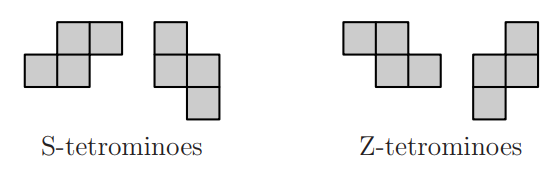
\includegraphics[width=0.3\textwidth]{tetrominos.png}

\end{questions}
\end{document}